The library consists of two main layers on the client side. An upper layer
to implement the RVM-specific logic and a lower-layer remote memory (RMEM)
backend to implement low-level transport and atomicity. This relationship is
described in Figure \ref{fig:lasagna}. This modularization allows for a number of
different backends to be tried independently of user code and the RVM layer.
This enhances portability and simplifies future efforts to improve performance
or semantics.

\begin{figure}[t]
\begin{center}
\resizebox{\columnwidth}{!}{%
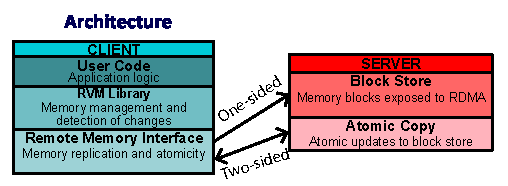
\includegraphics[scale=0.80]{lasagna.pdf}
}
\end{center}
\caption{RVM lasagna diagram}
\label{fig:lasagna}
\end{figure}

\subsection{The RVM API}

The RVM API consists of the following functions.

\begin{verbatim}
    rvm_cfg_create() / rvm_cfg_destroy()
\end{verbatim}

The \verb|rvm_cfg_create()| function sets up a connection to the remote node and, if necessary, recovers remote memory left over from a previous (failed) run of the application. The RVM configuration object returned by \verb|rvm_cfg_create()| is used in all the other commands. The \verb|rvm_cfg_destroy()| object cleans up the configuration object and closes the connection to the remote node.

\begin{verbatim}
    rvm_alloc() / rvm_free()
\end{verbatim}

    The \verb|rvm_alloc()| functions allocates memory both locally and on the remote node. Any modifications to the local pages allocated by \verb|rvm_alloc()| are automatically detected and copied to the remote node at commit time. \verb|The rvm_free()| function releases the local and remote memory allocated by \verb|rvm_alloc()|.

\begin{verbatim}
    rvm_txn_begin() / rvm_txn_commit()
\end{verbatim}

    All operations on recoverable memory (alloc, free, read, and write) should occur between a call to \verb|rvm_txn_begin()| and a call to \verb|rvm_txn_commit()|. When \verb|rvm_txn_commit()| is called, all memory pages that have been modified since the last call to \verb|rvm_txn_begin()| will be copied over to the remote node. The client then requests the remote node to atomically commit the modifications.




\subsection{The Remote Memory Layer}

Underlying the RVM API is the remote memory (RMEM) layer, which provides the
basic operations that RVM uses to communicate with the backing data store.
The essential operations in the RMEM layer are \texttt{put()}, \texttt{get()},
\texttt{malloc()}, \texttt{free()}, and \texttt{atomic\_commit()}.


\subsection{Infiniband Backend}

Our primary backend uses Infiniband Remote Direct Memory Access (RDMA) to talk
to a server managing a large pool of memory. At startup, the remote memory
server maps in a large block of system memory. The server then listens for
connections over the Infiniband fabric. When a client connects, the server
pins the memory in the page table and registers it with the infiniband drivers.
Registering with the infiniband drivers provides a local key and a remote key.
The server transmits the remote key and starting address to the client.
This allows the client to perform one-sided RDMA operations to the remote
memory without the server's mediation.

The \texttt{put()} and \texttt{get()} commands are implemented using one-sided
RDMA writes and reads. The other commands are implemented using two-sided sends
and receives. For these commands, the client and server each allocate two
message structs: one for sends, and one for receives. In a two-sided
transmission, the recipient first posts a receive request to the Infiniband
driver. This receive request specifies the local key and address of the receive
struct. When the sender posts a corresponding send request using the local key
and address of its send struct, the infiniband drivers copy the data from the
sender's send struct to the recipient's receive struct and notify sender and
recipient of the operation.

\begin{figure}
    \includegraphics[width=0.9\linewidth]{ib-backend-arch.pdf}
    \caption{IB Backend Architecture}
    \label{fig:ib-backend-arch}
\end{figure}

\subsubsection{Allocation}

The \texttt{malloc()} operation is implemented by sending an ALLOC request to
the server. When it receives this request, the server will allocate a block of
memory form the memory pool and mark it with the given tag.  The server then
sends a MEMRESP message back to the client containing the starting address of
the allocated block.

The \texttt{free()} operation is implemented by sending a TXN\_FREE request to
the server. A key feature of the IB backend is that the server does not
immediately perform a free operation when it receives the TXN\_FREE message.
Instead, it puts the free operation in a queue, which will be processed during
an atomic commit. This way, the free operation is transactional. Once the
server receives the message and queues the free operation, it sends a TXN\_ACK
message back to the client, allowing the client to send another command.

There are also MULTI\_ALLOC and MULTI\_TXN\_FREE requests which can encode up
to 20 allocation or free requests (this number if configurable at compile
time). The server responds to a MULTI\_ALLOC request with a MULTI\_MEMRESP
response, which contains an array of addresses, one for each tag in the
MULTI\_ALLOC request. The server responds to MULTI\_TXN\_FREE with a TXN\_ACK.

\subsubsection{Commit}

The \texttt{atomic\_commit()} operation involves two different message types.
The first is the MULTI\_TXN\_CP message, which instructs the server to copy a
set of source blocks to a set of destination blocks. However, as with
TXN\_FREE, the copy does not occur immediately. When the client sends the
server a TXN\_GO request, the server performs all requested copies and frees.
In our failure model, we assume that the server will not crash. So even if the
client crashes after sending TXN\_GO, the copies and frees will still be
performed to completion. If the client crashes before sending TXN\_GO, all of
the outstanding copy and free requests will be flushed and no changes will
occur.

\subsubsection{Recovery}

If a client reconnects after a crash, the IB server transmits the tag to
address mappings left over from the previous run to the client. The mappings
are transmitted to the client in groups of twenty through TAG\_ADDR\_MAP
messages. The client acknowledges each TAG\_ADDR\_MAP message with a
STARTUP\_ACK message.


\subsection{RAMCloud Backend}

% Ramcloud Backend

\begin{figure}[t!]
\begin{center}
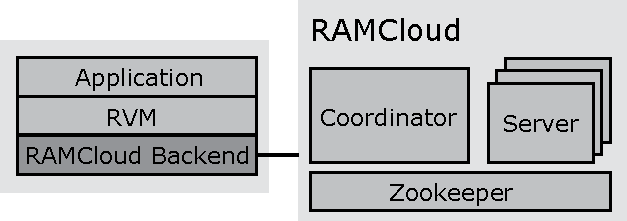
\includegraphics[scale=0.60]{graphs/ramcloud_backend_design_final.pdf}
\end{center}
\caption{RAMCloud backend layer operating along side RAMCloud.}
\label{fig:ramcloud_backend_design}
\end{figure}

To investigate the performance and suitability of a key-value store as a block device we developed a software layer on top of RAMCloud, a low-latency key-value store.
In RAMCloud, blobs of memory (values) are identified by keys (strings). When running, RAMCloud is composed of three main executing instances: a coordinator, a server and Zookeeper (see Figure~\ref{fig:ramcloud_backend_design}).
Each server is responsible for storing and serving data (values). The coordinator is responsible for keeping track of all servers alive and for keeping track of where data is stored in the system.
A Zookeeper instance is used for leader election and for storing configuration data.

Because RAMCloud's data is referenced by keys this layer keeps a map structure that associates each tag to a key. This means that each recoverable memory region can be uniquely identified by a key.

To provide atomicity and durability of the tag/key mapping, this backend keeps a special entry in RAMCloud with each tag-key association. This table is read each time the software layer is started and written once for each commit. This entry can be atomically written with a sngle {\emph put} operation.


\begin{figure}[t!]
\begin{center}
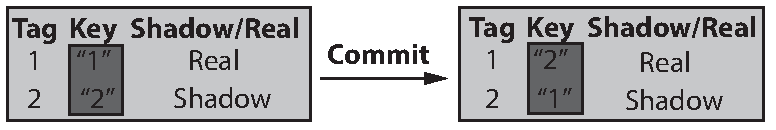
\includegraphics[scale=0.60]{graphs/ramcloud_backend_commit.pdf}
\end{center}
\caption{Diagram of tag/key mapping transformation during commit for a single memory region.}
\label{fig:ramcloud_backend_commit}
\end{figure}

\subsection{RAMCloud Backend}
\begin{figure}[t!]
\begin{center}
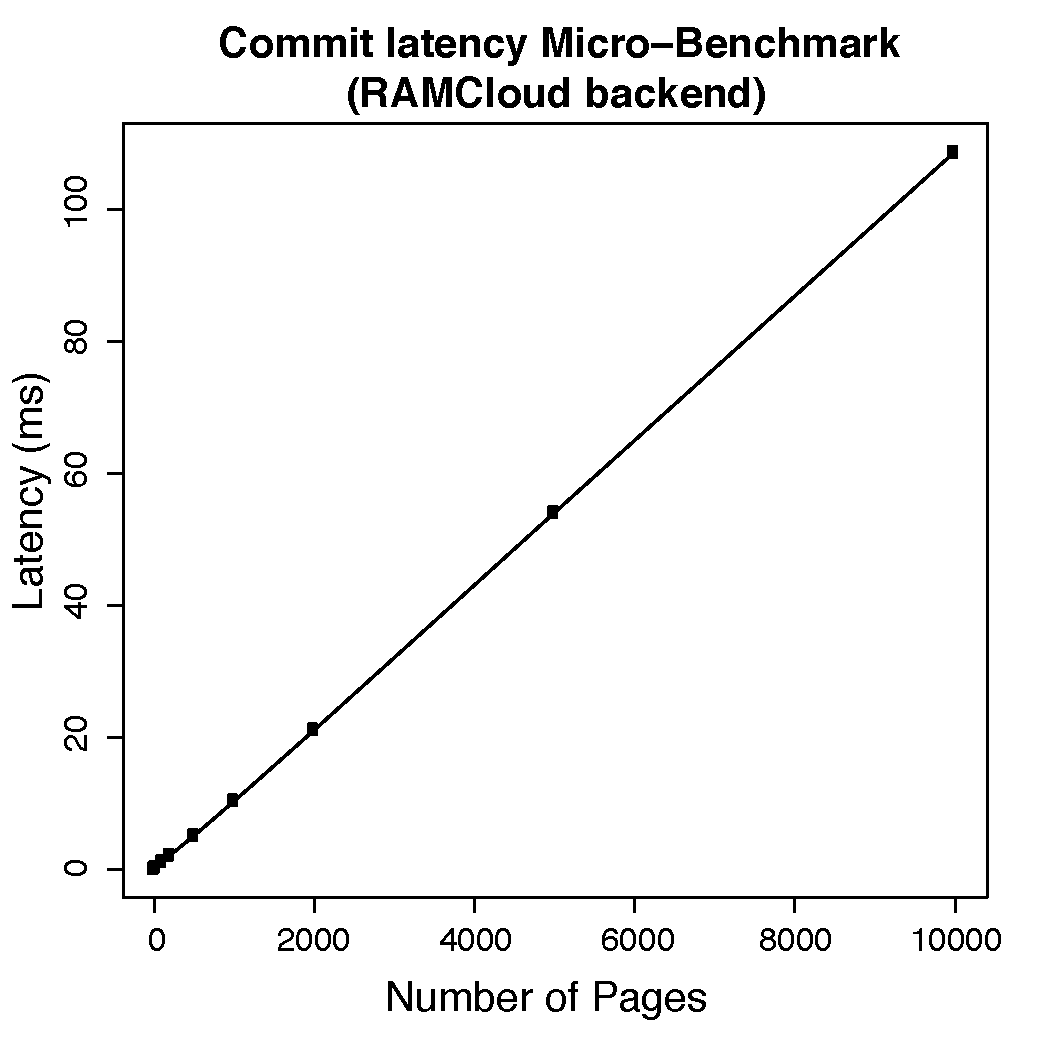
\includegraphics[scale=0.40]{graphs/commit_time_rc_latencies.pdf}
\end{center}
\caption{Commit time micro-benchmark when using the RAMCloud backend}
\label{fig:rc-commit-ubm}
\end{figure}

\begin{figure}[t!]
\begin{center}
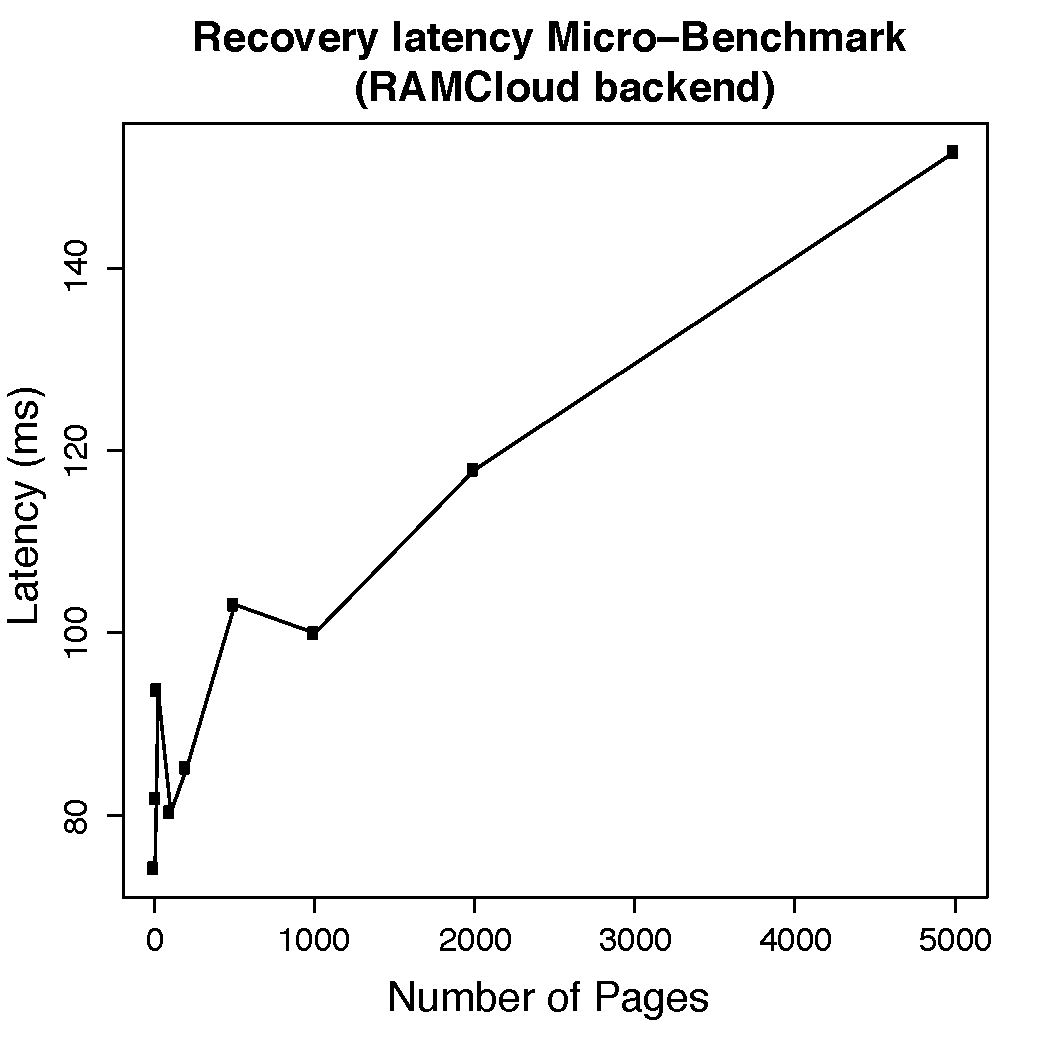
\includegraphics[scale=0.40]{graphs/recovery_time_rc_latencies.pdf}
\end{center}
\caption{Recovery time micro-benchmark when using the RAMCloud backend}
\label{fig:rc-recovery-ubm}
\end{figure}


The RMEM's layer operations are implemented in the following way:

\paragraph {\bf Connect} During connection the backend creates a RAMCloud client instance that is responsible for establishing a connection to the RAMCloud server.
If it is not the first time this connection is performed, i.e., if the client is under recovery, the backend recovers each tag-key mapping.
Otherwise, this layer initializes a RAMCloud table and stores an empty master entry in the RAMCloud's server.
\paragraph{\bf Allocate} During allocation, first the backend creates a key that identifies the memory being allocated in the RAMCloud server. Secondly, RAMCloud initializes this memory.
\paragraph{\bf Write} To write a memory region (identified by a tag) the backend fetches the tag's corresponding key and issues a {\emph put } operation with that key and corresponding data.
\paragraph{\bf Read} Likewise, to read a memory region the backend issues a {\emph get} operation with the tag's corresponding key. The data read from RAMCloud is copied to the final destination.
\paragraph{\bf Commit} To perform commit, the backend constructs a new master entry where each tag points to the key of the shadow memory being committed (see Figure~\ref{fig:ramcloud_backend_commit}). Likewise, the tag for each of the shadow
memory regions is made to point to the key of the old memory region (rephrase). Once this master entry is constructed in the backend, it is written atomically to RAMCloud.
\paragraph{\bf Disconnect} To disconnect, the backend clears the main data structures (e.g., local tag-key map).\\

Our design is simplified by the fact that our framework only replicates data to a single node. This means that we do not have to coordinate replicas.

